\documentclass[12pt, hyperref={bookmarks=false}, show notes]{beamer}
% Text
        \usepackage[T1]{fontenc}
        \usepackage[utf8]{inputenc}
        \usepackage[english]{babel}
        \usepackage[bitstream-charter]{mathdesign} % Serif font (Charter BT).
        \usepackage[scaled=0.84]{DejaVuSansMono} % Monospaced font.
        \def\sfdefault{SourceSansPro-TLF} % Sans serif font.
        \usepackage{textcomp}

% Maths
  \usepackage{amsmath}
  \usepackage{mathtools}
  \usepackage{siunitx}
  % Vector command
  \newcommand{\omatrix}[1]{\ensuremath{\boldsymbol{#1}}}

% Graphics
  \usepackage{graphicx}
  \usepackage[caption=false]{subfig}
        \usepackage{tikz}
  \usepackage{pgfplots}
  \pgfplotsset{compat=1.10}
        % ADD TIKZ LIBRARIES
  \usetikzlibrary{calc}
  \usetikzlibrary{arrows.meta}
  \usepackage{tikz-qtree}
  \usetikzlibrary{decorations.pathmorphing}
  \usetikzlibrary{matrix,shapes,positioning,fit}
  \usepgfplotslibrary{external}
  \tikzexternalize[prefix=graphics/tikz/]
  \tikzexternaldisable % Disable by default
  \usepackage{tabularx}
  \usepackage{pgfgantt}

        \usepackage{xcolor}
    \definecolor{color1}{cmyk}{100,50,0,0}   % blue
    \definecolor{color2}{cmyk}{0,80,100,0}   % vermillion
    \definecolor{color3}{cmyk}{97,0,75,0}    % blueish green
    \definecolor{color4}{RGB}{204,121,167}    % reddish purple
    \definecolor{color5}{RGB}{230,159,0}   % orange
   \usepackage{colortbl}
% Misc
\usepackage{booktabs}
\usepackage{enumerate}
\usepackage{pdfpages}
\usepackage{pgfpages}
\usepackage{setspace}
%\usepackage{multimedia}

\setbeamertemplate{navigation symbols}{}
\setbeamertemplate{caption}{\raggedright\insertcaption\par}
%\setbeamertemplate{bibliography item}[text]

%\usepackage{caption}
\usetheme{/amsterdam}
\date{October 11, 2016}

\usepackage{beamertheme/handoutWithNotes}
% Uncomment for handouts. Add \documentclass[12pt,handout]{beamer}
%\pgfpagesuselayout{4 on 1 with notes}[a4paper,border shrink=5mm]
% Comment for handouts.
\setbeameroption{show notes on second screen=right}

% Table of content dybde (0-index)
%\setcounter{tocdepth}{1}

% BibLaTeX
%\usepackage{csquotes}
%\usepackage[
%backend=bibtex,
%citestyle=numeric,
%bibstyle=numeric,
%maxcitenames=3,
%maxbibnames=99,
%url=true]{biblatex}
%\addbibresource{../rapport/references/refs.bib}
%\addbibresource{extrasources.bib}
%\usepackage{../style/biblatex_custom_formatting}

\graphicspath{{graphics/}{../../Report/graphics/}}

\begin{document}

%\captionsetup[figure]{font=small,singlelinecheck=off,justification=raggedright}

\title[Sentiment Knowledge Discovery in Twitter
Streaming Data]{TrashVision}
\author[\insertframenumber /\inserttotalframenumber]{SW703E15}

\begin{frame}
\Huge Sentiment Knowledge Discovery in Twitter
Streaming Data\\
\small International conference on Discovery science 2010, Albert Bifet and Eibe Frank\\
\end{frame}

\begin{frame}
  \frametitle{Contents}
  \tableofcontents
  \note{
  \begin{itemize}
    \item Background
    \item Related Work
    \item Theory
    \item Evaluation
    \item Result
  \end{itemize}
}
\end{frame}

% PUT INPUTS HERE
\section{Introduction}

\begin{frame}
     \begin{center}
     	\huge Introduction
     \end{center}
\end{frame}

\begin{frame}
\frametitle{Roles}
Roles are a method us to analyse networks
\begin{itemize}
\item Graph similarity 
\item Network modelling 
\item Visualization 
\end{itemize}
\end{frame}

\begin{frame}
\frametitle{Problem of Roles}
\begin{itemize}
\item Roles are network-specific giving it limited comparative options with other networks with another set of roles
\item In dynamic networks it is possible for roles to change or disappear over time
\end{itemize}
\end{frame}

\begin{frame}
\frametitle{The Goal of the Article}
The purpose of this paper is to present a novel method that uses features based on interaction patterns and structural positions of a users to:
\begin{itemize}
\item Find roles independent of dataset
\item Find roles that persists over time
\end{itemize}
This method should utilize the latent factors to identify the feature structure of the roles.

\note{
What is the article trying to do\\
Persistent roles consisting over time and datasets based on features.
}
\end{frame}






\section{Related Work}
%Context
In their work on aggregation of search queries, Dwork et al presented 4 Markov Chain(MC) methods.

To Dwork et Al, the idea of MC that the current state impacts future states were useful to get a better aggregation and provide a better interplay between candidates by comparing all candidates against each other. 

%Enhancement of other heuristics
It was their belief that this property of MC provided a natural extension to common aggregation methods such as Borda Count\note{First mention? BC?}.

Of the four methods presented, \MC managed to achieve some of the best results when scored on distance measures such as Kendall distance or Spearman's footrule, so of the four \MC will be our focus in this article.\cite{rank:aggregation}
\section{Methodology}

\begin{frame}
\begin{center}
     	\huge Methodology
     \end{center}
\end{frame}

\begin{frame}
\frametitle{The Approach}
\begin{figure}
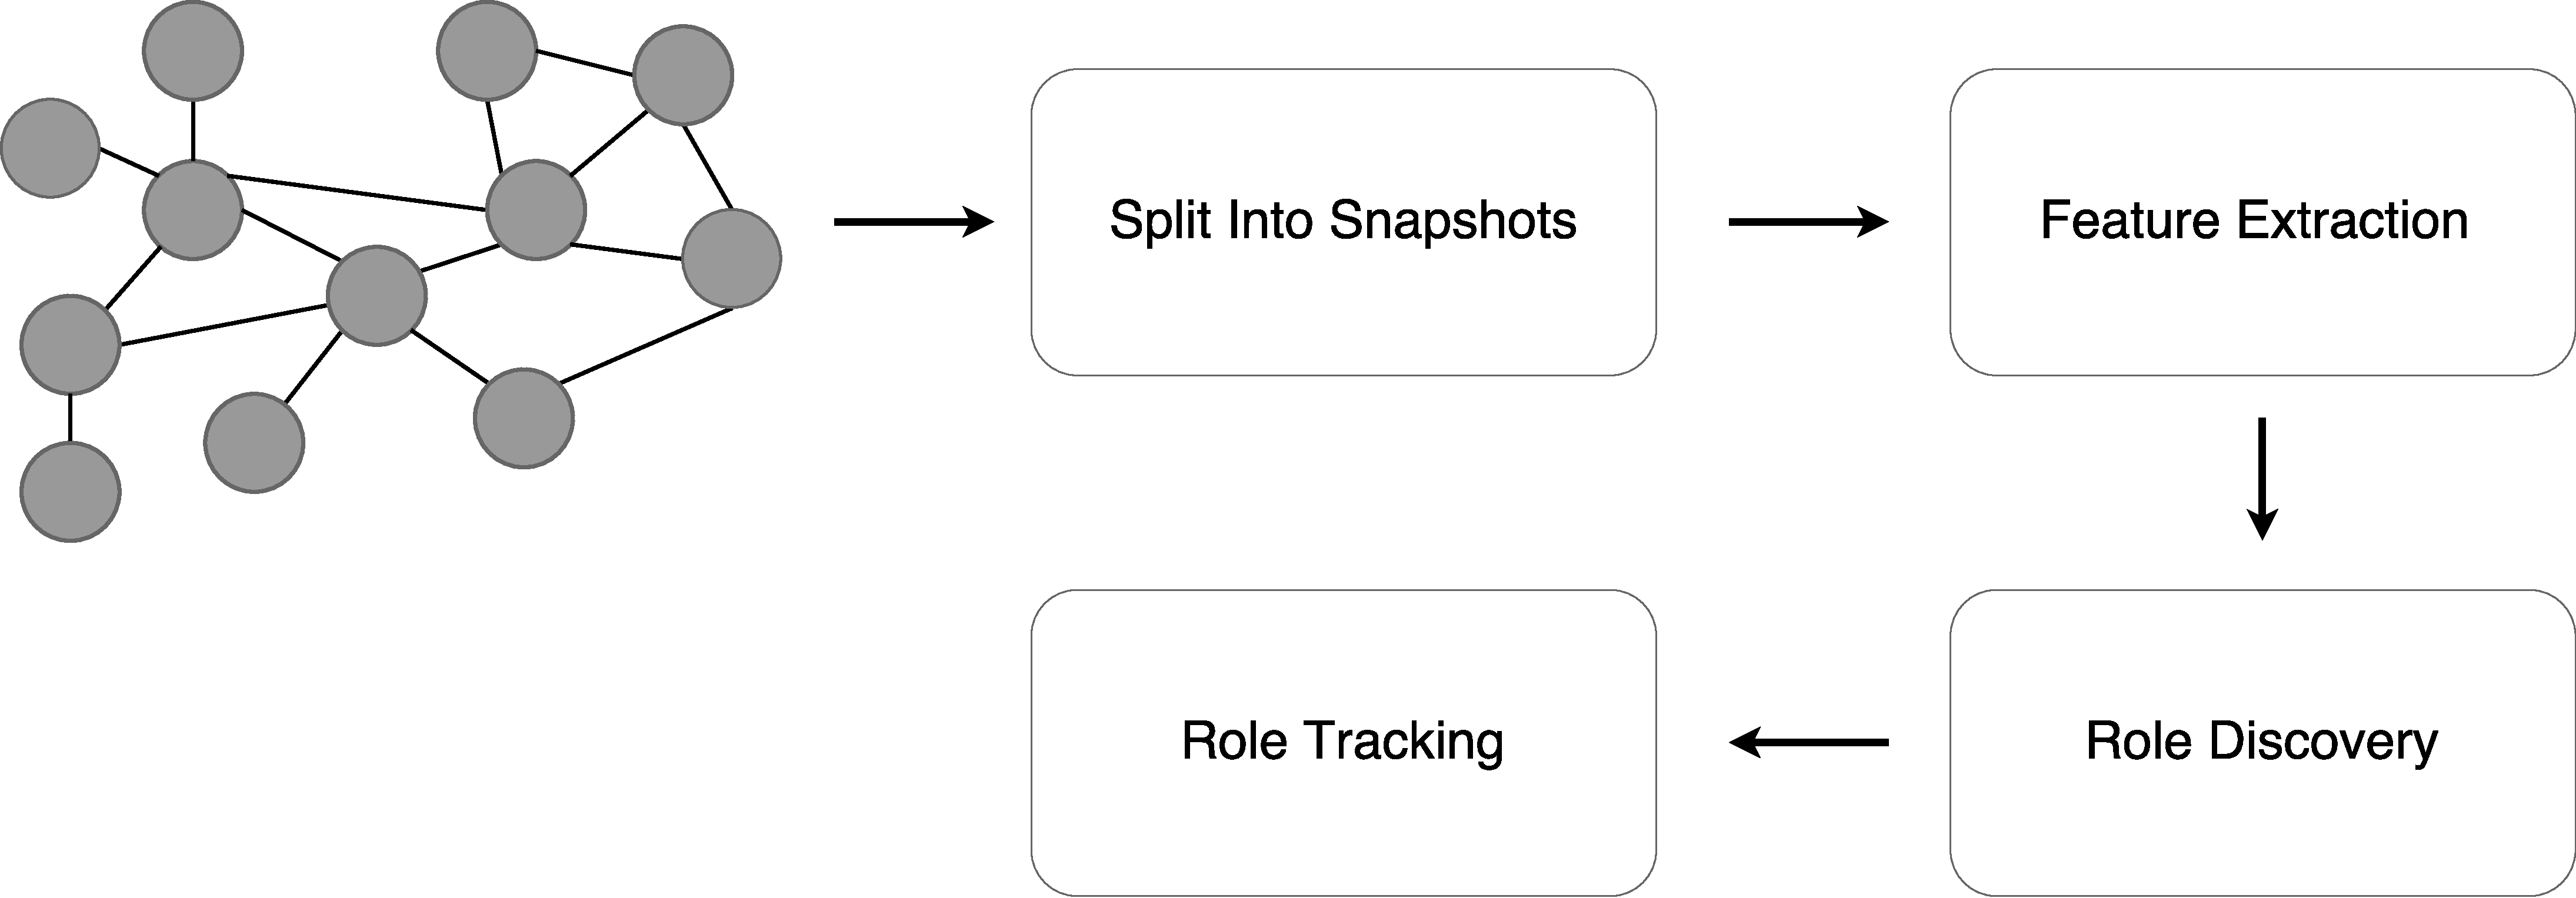
\includegraphics[scale=0.14]{graphics/setup.pdf}
\end{figure}
\note{Feature-based approach}
\end{frame}

\begin{frame}
\frametitle{The Data}
\begin{columns}
	\begin{column}{0.45\textwidth}
		Datasets:
			\begin{itemize}
				\item Facebook - Wall posts from one user to another
				\item Scratch - Comments on uploaded programming projects 
			\end{itemize}
			
		Directed, timestamps.
		\end{column}
		\begin{column}{0.55\textwidth}
			\begin{figure}
				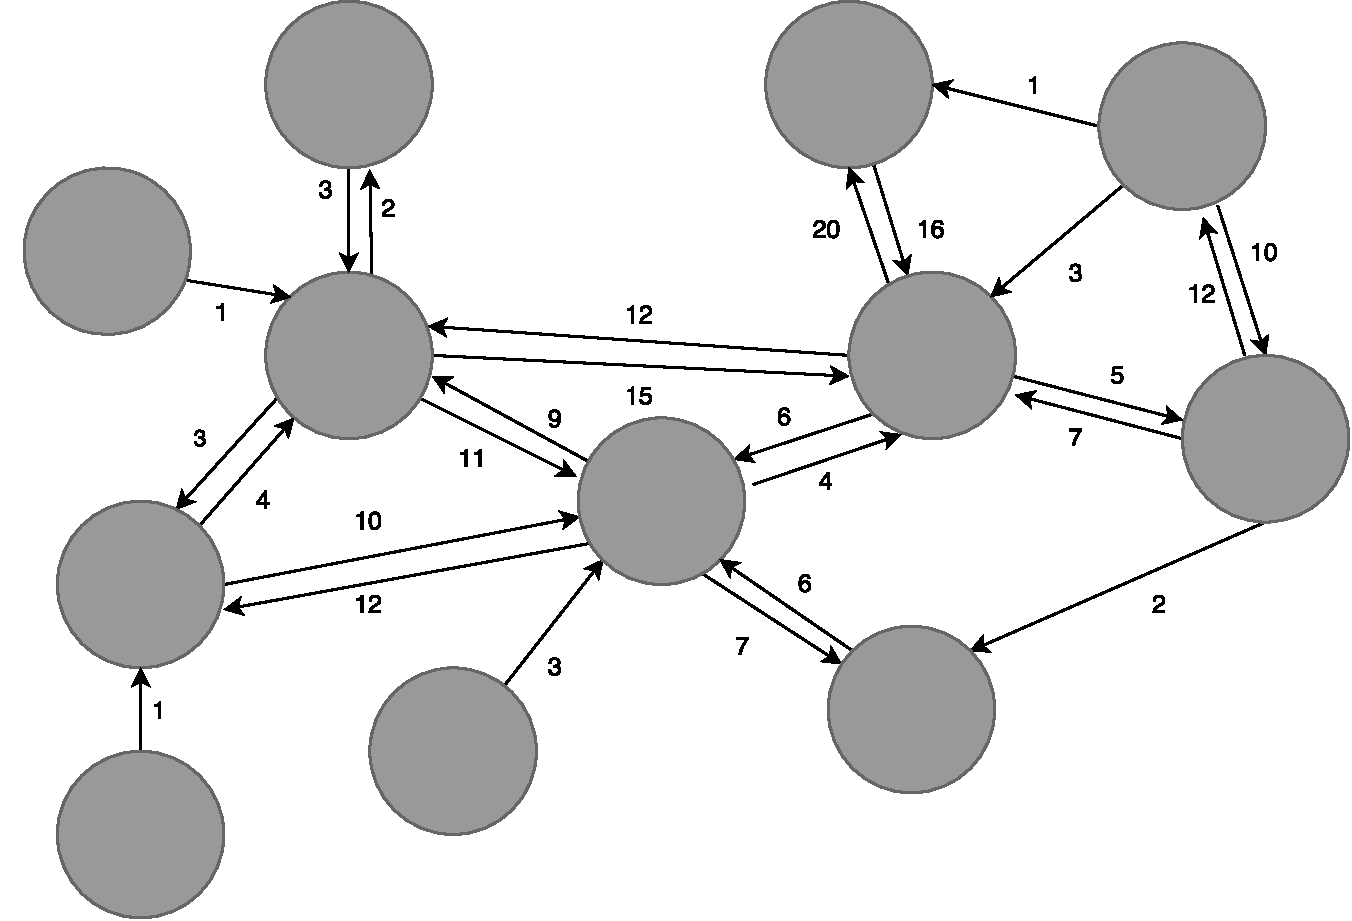
\includegraphics[scale=0.24]{graphics/directed_network.pdf}
			\end{figure}
		\end{column}
	\end{columns}
\end{frame}

\begin{frame}
\frametitle{Snapshot Split-up}
The dataset is split into a total of 26 snapshots:
\begin{itemize}
\item 7 from facebook
\item 19 from Scratch
\end{itemize}

Non-overlapping

Same length = observation window $\Omega$.

Something with node interaction being smaller than Omega. (90th percentile?)


\end{frame}

\begin{frame}
\frametitle{Feature Selection}
12 features based upon the graph.

	\begin{columns}
		\begin{column}{0.5\textwidth}
			\begin{figure}
				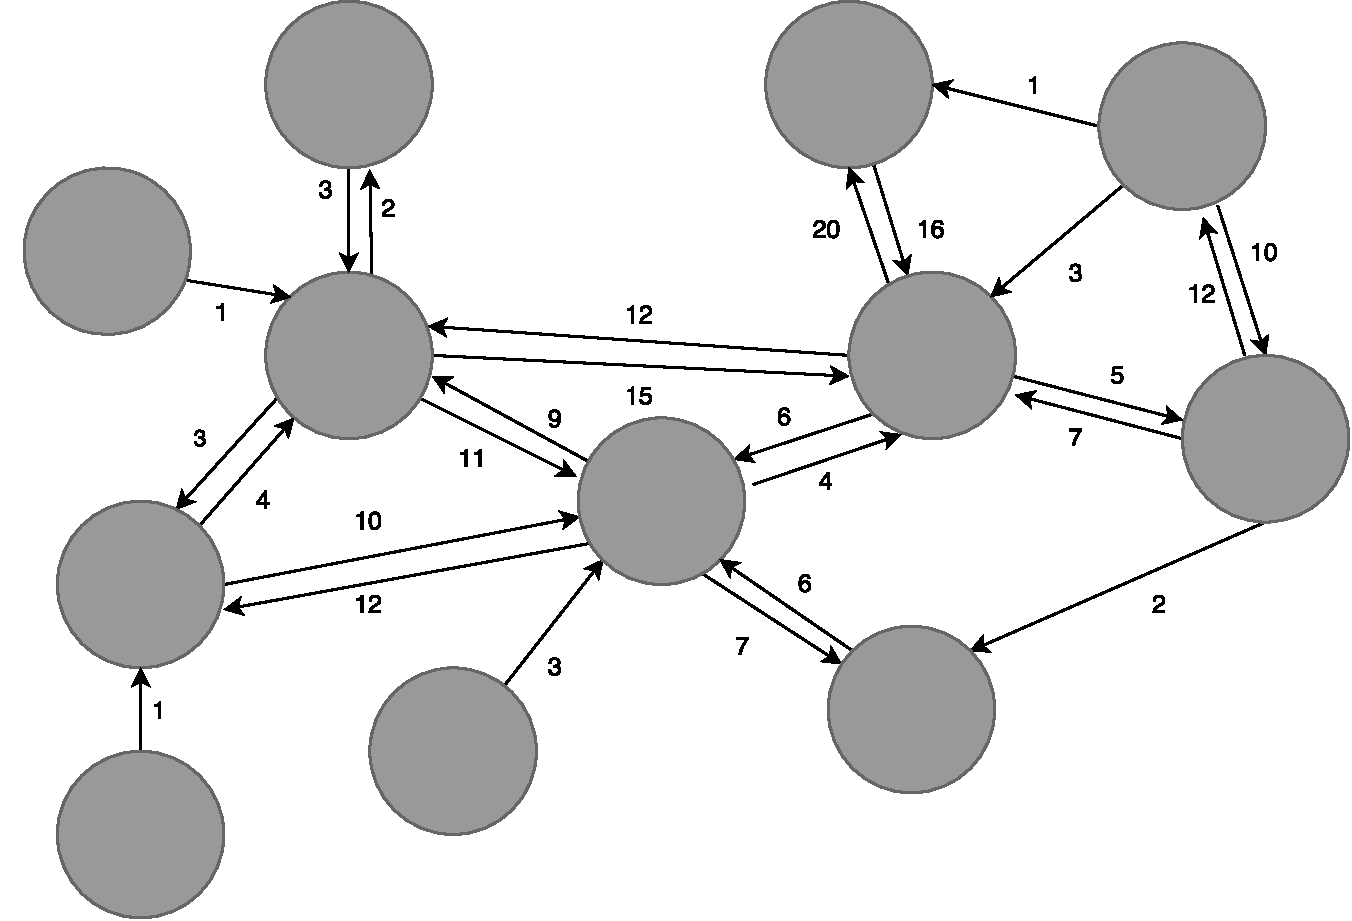
\includegraphics[scale=0.27]{graphics/directed_network.pdf}
			\end{figure}
		\end{column}
		\begin{column}{0.5\textwidth}
			\begin{table}
				\begin{tabular}{"l"}
				\thinhline
					In-degree				\\ \thinhline
					Out-degree				\\ \thinhline
					Weighted in-degree		\\ \thinhline
					Weighted out-degree		\\ \thinhline
					Reciprocity				\\ \thinhline
					New activity			\\ \thinhline
					Social strategy			\\ \thinhline
					Betweenness centrality	\\ \thinhline
					PageRank				\\ \thinhline
					Weighted PageRank		\\ \thinhline
					Transitivity			\\ \thinhline
					Weighted transitivity 	\\ \thinhline
				\end{tabular}
			\end{table}
		\end{column}
	\end{columns}

\end{frame}

\begin{frame}
\frametitle{Feature Example}


\begin{columns}
		\begin{column}{0.5\textwidth}
			\begin{figure}
				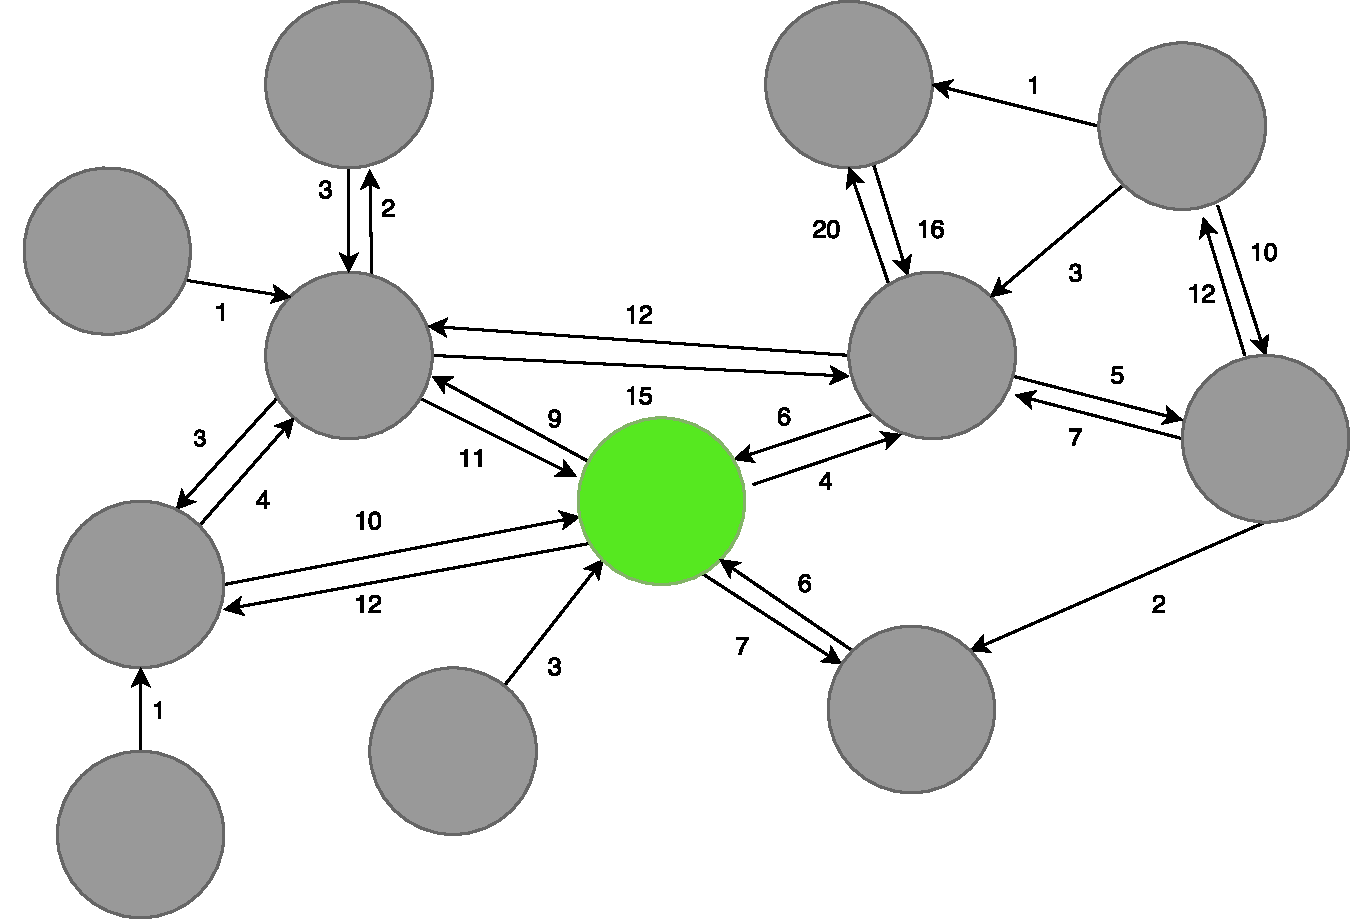
\includegraphics[scale=0.27]{graphics/directed_network_example.pdf}
			\end{figure}
		\end{column}
		\begin{column}{0.5\textwidth}
			\begin{table}
				\begin{tabular}{"l"l"}
				\thinhline
					In-degree				& 5		\\ \thinhline
					Out-degree				& 4		\\ \thinhline
					Weighted in-degree		& 36	\\ \thinhline
					Weighted out-degree		& 32	\\ \thinhline
					Reciprocity				& 4		\\ \thinhline
					New activity			& 0		\\ \thinhline
					Social strategy			& 0		\\ \thinhline
					Betweenness centrality	& 38.7		\\ \thinhline
					PageRank				& 0.21	\\ \thinhline
					Weighted PageRank		& -		\\ \thinhline
					Transitivity			& $\frac{1}{3}$		\\ \thinhline
					Weighted transitivity 	& -		\\ \thinhline
				\end{tabular}
			\end{table}
		\end{column}
	\end{columns}

\end{frame}

\begin{frame}
\frametitle{Role Discovery and Membership}

\begin{columns}
	\begin{column}{0.5\textwidth}
		\begin{block}{\small Non-negative Matrix Factorization}
			$X \approx UV$
		\end{block}
	\end{column}
	\begin{column}{0.5\textwidth}
	\end{column}
\end{columns}
\begin{figure}
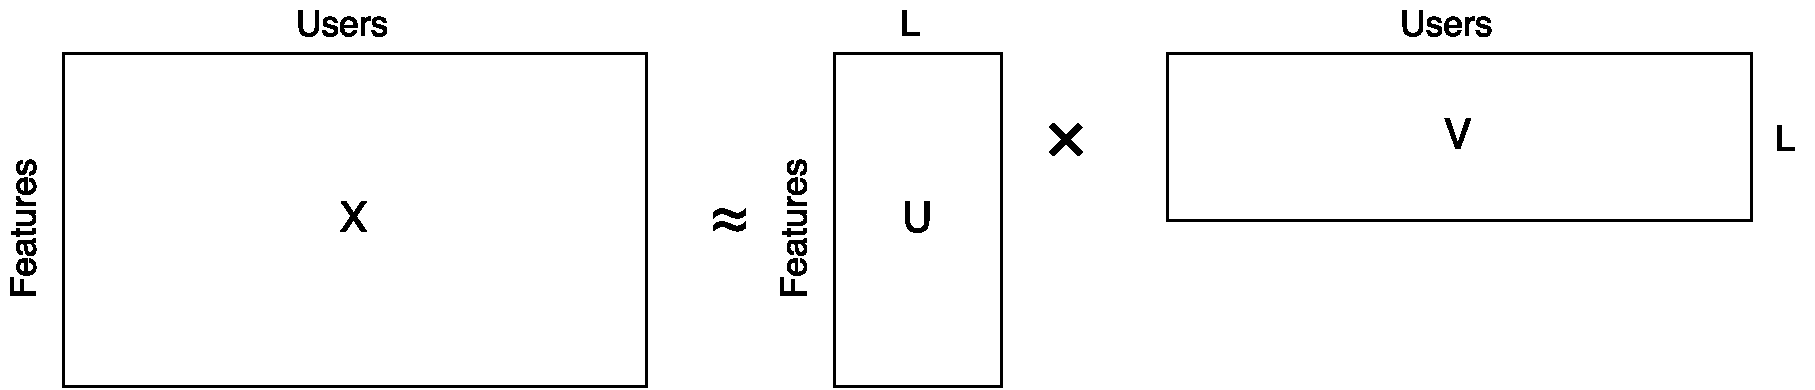
\includegraphics[scale=.3]{graphics/nmf}
\end{figure}

\note{
\begin{itemize}
\item Frobenius NMF updated with euclidean distance
\item U and V are initialized with left and right matrix from nndsvd (Modified svd)

\end{itemize}
}
\end{frame}

\begin{frame}
\frametitle{Selection of L}
\begin{block}{\small Root Mean Squired Error}
$RMSE = \sqrt{\frac{1}{|X|} \sum\limits_{(u,f) \in X}(X_{u,f}-X'_{u,f)}}$
\end{block}

\end{frame}

\begin{frame}
\frametitle{Tracing Roles}
The sim between snapshots. 
\end{frame}
\section{Evaluation}

\subsubsection{Dataset}\label{sec:dataset}
We used the MovieLens 100k dataset published by GroupLens in 1998\cite{movielens100k}. MovieLens 100K contains 100.000 ratings between 1 to 5 collected from 943 users across 1682 movies. With room for approximately one and a half million ratings, the 100k rating dataset is sparse. We used rating prediction to populate the rating matrix.

\subsubsection{Individual Recommendations}\label{sec:individualrecommendation}
For rating prediction, we used the library called MyMediaLite\cite{mymedialite}. MyMediaLite is a library for .NET that holds a bundle of recommendation methods for both item recommendation and rating prediction. We will be using the library, because this gives a tested foundation that is easy to reproduce for testing other aggregation methods and the focus of our paper lies in testing the aggregation methods.

Among the methods provided by MyMediaLite, SVD++ is one of the best performing on the 100k dataset on their own records using the parameters in Table \ref{tbl:svdpp}\footnote{www.mymedialite.net/examples/datasets.html}. For the sake of convenience we are using the same parameters as they are proven to be efficient.

\begin{table}[H]
	\centering
	\begin{tabular}{|l|l|}\hline
		Latent Factors & 50 \\
		Regularization & 1	\\
		Bias Regularization & 0.005	\\
		Learning Rate & 0.01 \\
		Bias Learning Rate & 0.07 \\ 
		Number of iterations & 50 \\
		Frequency Regularization & True \\\hline
	\end{tabular}
	\caption{Parameters values for the SVD++ component}
	\label{tbl:svdpp}
\end{table}

\subsubsection{Group Generation}\label{sec:groupgeneration}
For the aggregation we made groups consisting of 4, 8, 12, 16, 20, and 40 users from the MovieLens 100K dataset. This allows us to further the findings by Baltrunas et al\cite{Baltrunas:2010:GRR:1864708.1864733}, who had group sizes from 2 to 8.

Given that the dataset contains 943 users, we limited our group size to 40, as to not have any groups containing more than 5\% of all the users. This ensured some amount of diversity in the group. 40 is also ten times the size of our smallest group, enough to indicate the trend for the quality of recommendations. The groups were created of randomly picked users, and the same user can appear in multiple groups, but never in the same group twice.
\section{Results}

\begin{frame}
\begin{center}
     	\huge Results
     \end{center}
\end{frame}

\begin{frame}
\frametitle{The Roles}

\begin{table}
\begin{tabular}{"l"l|}
\hline
\rowcolor{HeadBlue}
\color{white}Role 		&	\color{white}Feature Characteristics\\\hline 
Popular					&	In-degree, Betweenness, PageRank 	\\\thinhline
\rowcolor{LightBlue}
Friendly				&	Out-degree							\\\thinhline
Reciprocated			&	Reciprocity							\\\thinhline
\rowcolor{LightBlue}
Explorer				&	Social Strategy						\\\thinhline
Community Member		&	Transitivity						\\\thinhline
\rowcolor{LightBlue}
Active Community Member &	Weighted transitivity				\\\hline

\end{tabular}
\end{table}
\end{frame}

\begin{frame}
\frametitle{Feature Representation of the Roles}
\begin{figure}
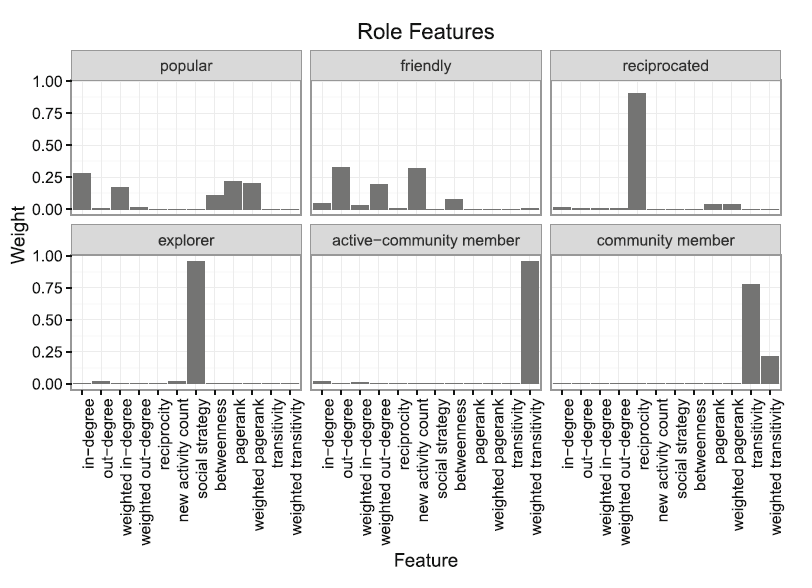
\includegraphics[scale=.5]{roles}
\end{figure}
\end{frame}

\begin{frame}
\frametitle{Interaction Preferences}\centering

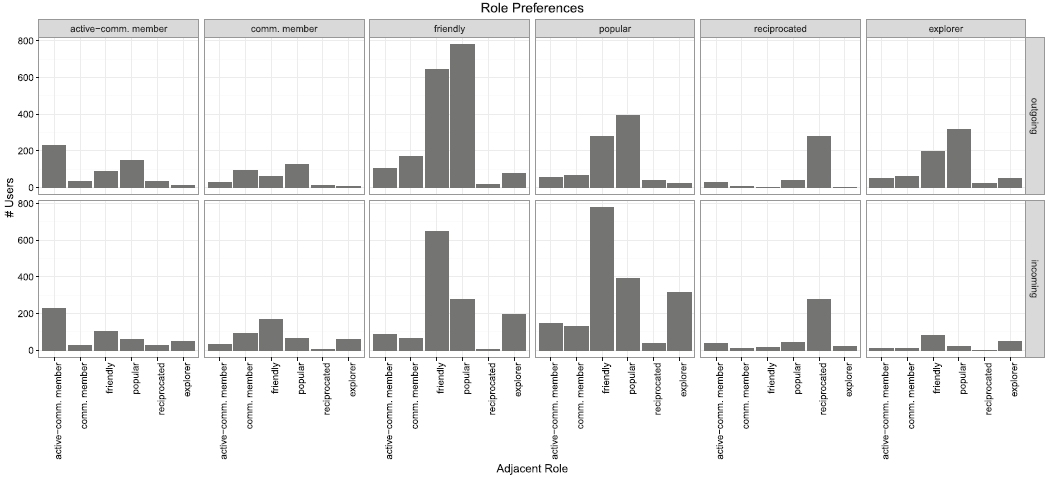
\includegraphics[scale=.42]{relations}

\note{affinity analysis}
\end{frame}

\begin{frame}
\frametitle{Evidence of Roles Dependence on Network Structure}
\begin{figure}
	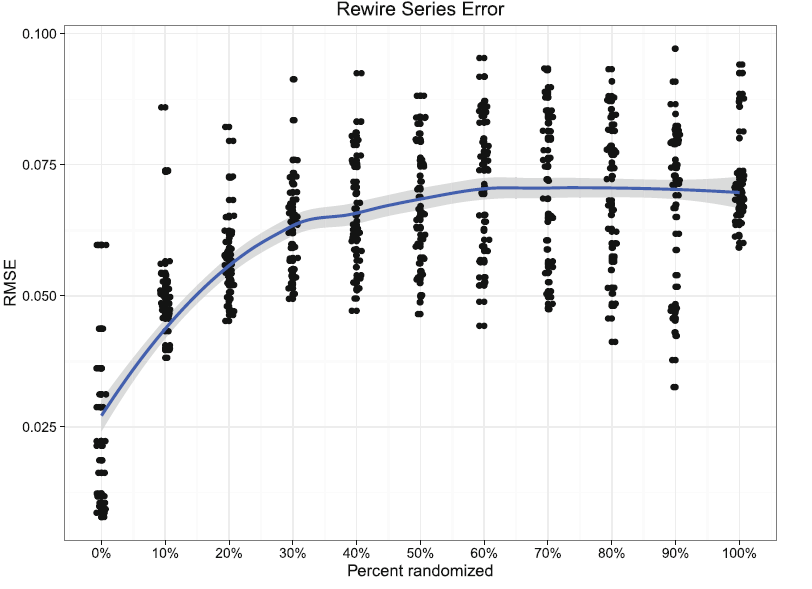
\includegraphics[scale=.5]{evidence}
\end{figure}
\end{frame}

\section*{}

\end{document}
